\chapter{Ansible}

Ansible on tarkoitettu palvelinten konfiguraation hallinnoimiseen, palveluiden hallinnointiin ja esimerkiksi web-palveluiden käyttöönottoon ja asentamiseen. Ansiblella voidaan esimerkiksi asentaa kehitys- että tuotantoympäristöön tarvittavat riippuvuudet helposti ja paremmin kuin esimerkiksi shell-skripteillä. Nykyään on myös hyvä tapa tehdä kehitys- että tuotantonympäristöstä mahdollisimman samanlaisia, jotta ympäristöjen erilaisuuksista ei tule ongelmia. Ansiblessa pystyy helposti uudelleen käyttämään siihen määriteltyjä asennustehtäviä parametrisoimalla niitä. Esimerkiksi tietokantayhteys voi hieman poiketa tuotantoympäristössä. Kaikki nämä ja paljon muuta hoituu helposti Ansiblella.

Mietitään jälleen vertauskuvaa Subway-ravintolan perustamisesta. Kun laatikosta tullut robotti on rakentanut ravintolan liiketilan se aloittaa laitteiden asentamisen ja sisustamisen. Jos Erik haluaa myöhemmin esimerkiksi sisustaa ravintolan uudestaan ohjeiden mukaan ollakseen varma, että ravintolan on Subwayn johdon määritelmän mukainen, hänen täytyy kutsua robottia tekemään sisustus uudestaan. Tämä toiminpide täytyy tehdä viimeistään silloin kun Subwayn johto on muuttanut rakennusohjeita.

Vanha robotti tekisi tällöin sekä laitteiden asennuksen, että sisustuksen uudestaan, mutta se saattaa rikkoa paikkoja, koska se esimerkiksi sisustaisi kaiken uudestaan vaikka osa sisustuksesta olisikin jo paikoillaan. Tästä voi luonnollisesti koitua ongelmia ja pahimmassa tapauksessa robotin täytyy tuhota koko ravintola ja aloittaa alusta rakentaminen, laitteiden asennus ja sisustaminen. Toisaalta tämä ei haittaa, koska alusta asti rakennettu ravintola toimii aina. Ainostaan aikaa menee tällöin hukkaan.

Uusi robotti on fiksumpi kuin edellinen. Kun Erik haluaa varmistaa, että ravintola on vanhojen ohjeiden mukainen tai varmistaakseen, että uusimmat muutokset ovat tehty ravintolaan täytyy hänen jälleen kutsua robottia asentamaan ravintola. Ennen kuin uusi robotti alkaa asentaa mitään se tutkii ravintolaa ja kerää siitä tietoa. Kun tiedot on kerätty se aloittaa asentamisen. Esimerkiksi jääkaapin asennuken kohdalla robotti ensin tutkii onko jääkaappi jo asennettu ja jos se on niin se siirtyy seuraavaan asennukseen. Asennuksen päätteeksi robotti ilmoittaa Erikille kuinka monta asiaa asennuslistalta oli jo tehty ja kuinka monta asiaa muutettiin. Esimerkiksi: "10 kohdetta oli jo asennettu ja jääkaapin tilalle asennettiin jääkaappipakastin yhdistelmä".

\section{Ansiblen toiminta}

Ansiblen kaltaisia ohjelmia on muutamia, mutta Ansiblen suosio perustuu sen yksinkertaisuuteen ja keveyteen. Käyttääksesi Ansiblea tarvitset vain Pythonin, SSH-yhteyden kohdekoneeseen ja käyttäjän, joka voi suorittaa skriptejä kohdekoneella \cite{link:what-is-ansible}. Jotta Ansiblen käyttäminen olisi erittäin sujuvaa kannattaa kohdekoneelle lisätä SSH-avain, koska tällöin ei tarvita käyttäjätunnus salasana yhdistelmää kun otetaan yhteyttä kohdekoneeseen.

Jotta Ansible pääsee suorittamaan sille annettuja tehtäviä kohdekoneeseen, täytyy sen ensin ottaa SSH-yhteys kohdekoneeseen. Tämä ei vaadi client-koneelta yleisesti mitään lisäasetuksia. Kun yhteys on saatu kohdekoneeseen kerää Ansible tietoja siitä esimerkiksi käyttäjärjestelmän, mitä paketteja on jo asennettu yms. Sen jälkeen Ansible lähtee ajamaan sille määriteltyjä tehtäviä kohdekoneelle. Tehtävät määritellään playbookkeina, jotka sijaitsevat client-koneella \ref{fig:how-ansible-works}

\begin{figure}[h]
  \includegraphics[width=\textwidth]{how-ansible-works}
  \caption{Ansiblen toiminta}
  \label{fig:how-ansible-works}
\end{figure}

Tehtävä voi olla esimerkiksi palvelinohjelman kuten Apachen asentaminen, tiedoston kopioiminen tai tietokannan käynnistäminen. Ansible suorittaa sille annetut tehtävät määritellyssä järjestyksessä. Tehtävät kuvataan Ansiblen tarjoamilla moduuleilla. Moduuleita on niin paljon, että varmasti jokaiseen tarpeeseen löytyy oma. Ansiblelta löytyy hyvät dokumentaatiot kaikille moduuleille. Esimerkiksi tiedoston kopioiminen onnistuu helposti copy-moduulilla. Kun SSH-yhteys on luotu ja kohdekonetta on tutkittu, voidaan aloittaa tehtävien suorittaminen.

Kuvassa \ref{fig:how-ansible-loops-tasks} näytetään miten Ansible prosessoi sille annettuja tehtäviä. Ansible tarkistaa kaikkien tehtävien kohdalla onko muutoksia tapahtunut. Muutos tarkoittaa, että onko tehtävää suoritettu ollenkaan tai onko tehtävää muutettu sitten viime suorituksen jälkeen. Esimerkiksi jos Apachea ei ole asennettu ollenkaan niin suoritetaan tehtävä. Lisäksi jos viimeksi sama tehtävä on muutettu asentamaan NGINX Apachen sijaan niin suoritetaan tehtävä tällöinkin. Kun tehtävä on suoritettu tarkistetaan onko vielä tehtäviä jäljellä. Jos on niin jatketaan niiden suorittamista. Jos Ansible toteaa, että muutoksia ei ole eli esimerkiksi kyseinen ohjelma on jo asennettu, jatketaan suoraan tarkistamaan onko tehtäviä vielä jäljellä -osioon. Tätä silmukkaa jatketaan kunnes tehtäviä ei ole enään jäljellä.

Kun tehtävä ovat loppuneet antaa Ansible yhteenvedon tehtävistä. Se kertoo esimerkiksi kuinka monta tehtävää ei tarvinnut suorittaa (ei muutoksia) ja kuinka tehtävää suoritettiin (muutoksia oli).

Yksi Ansiblen hienoista ominaisuuksista on päivityksen peruminen. Jos äsken suoritettu asennus rikkoi kohdekoneen niin päivityksen voi vielä peruuttaa. Peruuttamisen avulla kehittäjät voivat huoletta viedä uusia ominaisuuksia tuotantoon ilman pelkoa, että kaikki menee hajalle. Aikaisemmin tällaisesta tilanteesta olisi voinut koitua erittäin suurta vaivaa saada kohdekoneen tila samaa kuin se oli aikaisemmin.

\begin{figure}[h]
  \centering
  \includegraphics[width=\textwidth, height=\textheight,keepaspectratio]{how-ansible-loops-tasks}
  \caption{Ansiblen tehtäväprosessointi}
  \label{fig:how-ansible-loops-tasks}
\end{figure}

\section{Ansiblen käyttäminen}

Ansiblen käytön aloittamiseksi se pitää asentaa osoiteen \url{http://docs.ansible.com/ansible/intro_installation.html} mukaan. Asennuksen jälkeen avaa komentorivi ja komenna \code{ansible -{}-version} ja jos Ansible kertoo nykyisen versionsa on Ansible asennettu oikein.

Seuraavaksi luodaan jälleen Vagrant virtuaalikone, mutta nyt siihen asennettavat ohjelmat ja riippuvuudet ei asenneta shell-skriptin vaan Ansible playbookin avulla. Jatketaan kuviossa \ref{listing:vagrant-final-apache-setup} olevaa Vagrantfileä.

Ensiksi korvataan shell-skriptin määrittelevä rivi, niin että määrittelemme riippuvuuksien asentajaksi Ansiblen. Kuviosta \ref{listing:vagrantfile-ansible} nähdään Ansiblen määrittely. Määrittelyssä kerrotaan Ansiblelle, että playbook löytyy tiedostosta "playbook.yml", joka on samassa kansiossa, jossa Vagrantfile on. Playbook sisältää kaikki tiedot virtuaalikoneen riippuvuuksien asentamiseen. Playbook-tiedosto on yksinkertainen YAML-tiedosto.

\begin{lstlisting}[
  label=listing:vagrantfile-ansible,
  language=Ruby,
  caption=Määritellään virtuaalikoneen riippuvuuksien asentajaksi Ansible,
  float=h
]
config.vm.provision "ansible" do |ansible|
  ansible.playbook = "playbook.yml"
end
\end{lstlisting}

Sitten luodaan playbook.yml tiedosto, joka on kuvattu kuviossa \ref{listing:base-playbook}. Kaikki YAML-tiedostot pitäisi aloittaa sijoittamalla kolme väliviivaa dokumentin alkuun. Tämä on YAML:n tapa kertoa, dokumentin alkukohdasta.

Ensin määritellään hostit eli mille kohdekoneille kyseinen playbook suoritetaan. Tässä tapauksessa voidaan määritellä kaikki kohdekoneet, koska Ansiblea käskytetään Vagrantin kautta, jolloin vain virtuaalikoneelle asennetaan riippuvuuksia \cite{link:comprehensive-ansible-tutorial}. Yleisesti kohteiksi ei laiteta kaikkia mahdollisia kohdekoneita. Kohteina normaalisti olisi esimerkiksi, dev (kehitysympäristö), staging (testausympäristö) tai production (tuotantoympäristö).

Määrittely true avaimelle "become" tarkoittaa, että kaikki playbookissa olevat tehtävät ajetaan root-oikeuksilla. Eli sama asia kuin lisäisi esimerkiksi asennuskomentojen eteen "sudo". Tällä tavalla ohjelmia voidaan ylipäätään asentaa kohdekoneille \cite{link:ansible-configuration-file}.

Jotta voidaan määritellä käyttäjätunnus, jolla tehtäviä ajetaan kohdekoneella täytyy määritelmälle "remote\_user" antaa arvo. Virtuaalikoneen tapauksessa arvoksi laitetaan vagrant, koska se on Vagrant virtuaalikoneiden oletuskäyttäjä.

\begin{lstlisting}[
  label=listing:base-playbook,
  language=Ruby,
  caption=Pohja Ansible playbookille,
  float=h
]
---
- hosts: all
  become: true
  remote_user: vagrant
  tasks:
    - name: Update apt cache
      apt:
        update_cache: yes
\end{lstlisting}

Kaikki tehtävät määritellään playbookkiin tasks avaimen kohdalle. Kuviossa \ref{listing:base-playbook} määritellään vain yksi tehtävä. Tehtävällä pitää olla jokin nimi. Nimi kannattaa kirjoittaa mahdollisimman ihmisystävälliseksi, koska nimi näkyy asennusprosessin aikana, mikä helpottaa tilanteen seuraamista. Kuviossa tehtävä on nimetty kyseisellä tavalla, koska tehtävässä päivitetään pakettityökalun välimuisti paketeista. Normaalisti välimuistin päivitys tehtäisiin komennolla \code{sudo apt-get update}. Sudoa ei tarvitse kirjoittaa mihkään, koska kaikki tehtävät suoritetaan sudo voimilla, koska aikasemmin kohtaa become määriteltiin true, joka nostaa kaikkii komentoihin sudo oikeudet.

Sitten tehtävälle pitää kertoa mitä Ansible moduulia se käyttää tehtävän suorittamiseen. Jos ei tiedä mitä moduulia kannattaa käyttää niin suosittelen Googlaamaan normaalin komennon nimen ja perään Ansible. Esimerkiksi kun etsii \code{apt-get update ansible} niin ensimmäisenä löytyy Ansiblen dokumentaatio apt-moduulista. Moduulin dokumentaatiosta nähdään, että pakettien välimuistin voidaan päivittää kuvion \ref{listing:base-playbook} osoittamalla tavalla.

\subsection{Node.js ympäristön luominen Ansiblella}

Seuraavaksi laajennetaan kuviossa \ref{listing:base-playbook} olevaa pohja playbookkia niin, että virtuaalikoneelle saadaan asennettua Node.js. Tavoitteena on myös asentaa pieni Node-palvelin, jota voidaan kutsua isäntäkoneen internetselaimesta.

Ensin katsotaan miten Node.js asennettaisiin normaalisti Ubuntulle (virtuaalikoneen käyttöjärjestelmäksi on valittu aikaisemmin Ubuntu). Kuviossa \ref{listing:install-node-with-shell-script} on esitetty asennus shell-skriptinä. Esimerkki shell-skriptistä näytetään, jotta saadaan varmasti kuva siitä mitä ollaan tekemässä. Shell-skriptissä ensin ladataan nodesourcen-sivuilta neljännen version skripti, joka suoritetaan samalla rivillä. Tämä skripti päivittää paikallisen nodejs paketin repositorion, joten kun se asennetaan saadaan uusin versio neljännestä Nodesta. Seuraavalla rivillä asennetaan Node.js pakettityökalulla. Viimeisellä rivillä asennetaan vielä apukirjasto, joka on yleisesti hyvä olla kun Noden kanssa ollaan tekemisissä.

\begin{lstlisting}[
  label=listing:install-node-with-shell-script,
  language=bash,
  caption=Node.js:n asennus shell-skriptillä,
  float=h
]
#!/bin/bash
curl -sL https://deb.nodesource.com/setup_4.x | sudo -E bash -
sudo apt-get install -y nodejs
sudo apt-get install -y build-essential
\end{lstlisting}

Seuraavaksi samat asiat, jotka shell-skripti tekee on tarkoitus kuvata Ansible tehtävälistana. Voidaan olettaa, että apt-moduulia tarvitaan taas, koska sama moduuli teki pakettien välimuistin päivityksenkin. Shell-skriptissä oleva curl ohjelma lataa internetistä tiedostoja ja sitä vastaava moduuli on get\_url. Lopuksi ladatun skriptin suorittamiseen käytetään moduulia shell.

Kuviossa \ref{listing:install-node-with-ansible} tasks-ominaisuuden alle on lisätty Node.js:n asennukseen tarvittavat moduulit. Kuviosta huomataan myös, että Noden asennus tehdään nyt melko monessa osassa. Ensimmäinen tehtävä lataa aiemmin mainitun Noden päivitysskriptin. Skripti laitetaan polkuun \code{/tmp}, koska kyseiseen kansioon laitetaan väliaikaisia tiedostoja. Seuraavaksi skripti suoritetaan ensin siirtymällä parametrilla \code{chdir} väliaikaisten tiedostojen kansioon ja sitten ajamalla skripti.

Seuraava tehtävä käyttää aikaisemmin nähtyä apt-moduulia. Usein asennettavia paketteja apt:n kautta on monta, joten olisi turhan runsassanaista kirjoittaa jokaiselle asennukselle oma tehtävä. Tästä syystä Ansible-skripteissä voi käyttää with\_items-avainta. Kyseinen avain on käytännössä taulukko ohjelmista, jotka halutaan asentaa. Sitten apt-moduulin name-avaimen kohdalle ei laitetakkaan yksittäisen paketin nimeä vaan \code{"\{\{ item \}\}"}. Näin asennetaan tarvittavat paketit: nodejs ja build-essential.

Lopuksi Noden päivitysskripti poistetaan file-moduulilla. State avaimen parametriksi annetaan tällöin absent.

Nyt playbook on valmis Node ympäristön luomiseen. Ajetaan siis komento \code{vagrant up}. Nyt Vagrant tekee samoja asioita mitä aikaisemmin esim asentaa Ubuntun, ohjaa portteja virtuaalikoneesta isäntäkoneeseen tms. Kun Vagrant on suorittanut perustehtävät se alkaa asentamaan Ansiblen avulla Nodea. Kuvassa \ref{fig:ansible-running} nähdään kun Ansible kertoo tehtävä tehtävältä mitä se on tekemässä.

Kuvasta huomataan, että shell provisionerin sijasta käytetään ansible provisiointi, niin kuin Vagrantfilessä määriteltiin. Ensiksi Ansible ilmoittaa mille kohdekoneille se ajaa tehtäviä. Tässä tapauksessa se on kaikki eli pelkästään virtuaalikone, koska muita ei ole saatavilla. Tästä eteen päin Ansible näyttää ihmisluettavan tekstin, jossa lukee sen hetkisen tehtävän nimi. Tehtävän ala puolella miten tehtävän suorituksessa tehtiin. Tila ok tarkoittaa, että tehtävää ei tarvinnut suorittaa. Kuvassa esimerkiksi pakettien päivitystehtävä ei suoritettu, koska paketit oli päivitetty jo aikaisemmin. Tällöin Ansible vain ohittaa tehtävän ja siirtyä eteenpäin.

Tehtävä, jossa ladataan Noden päivitysskripti on tilana changed, joka tarkoittaa, että pakettia ei ole ennen asennettu tai se on esimerkiksi asennettu ennen, mutta nyt se on jostain syystä poistettu. Ensimmäisellä kerralla tietysti ajettaessa syy on juuri asennettu virtuaalikone, johon ei ole vielä asennettu mitään.

Jos jokin tehtävistä epäonnistuu antaa Ansible tilaksi unreachable tai failed. Laitetaan tahallaan yksi tehtävä epäonnistumaan. Kuvassa \ref{fig:ansible-fails} näkyy virheellisen tehtävän tuloste. Virheviestissä näkyy, että Ansible yrittää ajaa tiedostoa, jota ei ole olemassa (node-setupdfg). Ansible ei myöskään suorita muita tehtäviä jos jokin niistä epäonnistuu.

Playbookin suoritettuaan Ansible antaa yhteenvedon, siitä kuinka tehtävät suoritettiin. Kuvassa \ref{fig:ansible-summary} näkyy Noden asennuksen yhteenveto. Yhteenvedossa lasketaan vain tehtävien eri tilat yhteen. Koska kaikki tehtävät menivät läpi voidaan olettaa että virtuaalikoneella on nyt uusin versio neljännestä Nodesta.

Siirrytään jälleen komennolla \code{vagrant ssh} virtuaalikoneen sisään. Tarkastetaan komennolla \code{node -v}, että Node on asennettu ja versio numero alkaa numerolla neljä.

\subsection{Node palvelimen luominen}

Luodaan projektin juureen tiedosto app.js, johon laitetaan pienen http-palvelimen koodi. Palvelimeen on tarkoitus ottaa yhteys internetselaimen kautta isäntäkoneelta.

Ennen koodin lisäämistä Vagrantfilestä pitää muuttaa projektin koodien synkronointi sijainti. Sijainniksi valitaan \code{/vagrant}. Lisäksi muutetaan virtuaalikoneen portti 8080 osoittamaan porttiin 3000 isäntäkoneessa. Kuviossa \ref{listing:final-node-vagrantfile} on lopullinen Node ympäristön Vagrantfile. Vagrantfilessä uudet muutokset saa voimaan esimerkiksi tuhoamalla virtuaalikoneen komennolla \code{vagrant destroy}, mutta useasti sitä ei haluta koko ajan tehdä, koska se vie aikaa. Ajamalla \code{vagrant reload} Vagrant pitää vanhan virtuaalikoneen tallella ja ajaa siihen muuttuneet kohdat Vagrantfilessä.

Nyt kun mennään takaisin virtuaalikoneen sisään ja siirrytään kansioon \code{/vagrant} niin siellä on kaikki projektin tiedostot. Lisätään tiedosto app.js, johon laitetaan Node-palvelimen koodit. Kuviossa \ref{listing:node-server} on app.js tiedoston sisältö. Koodissa ensin tuodaan http-moduuli, jonka avulla palvelin luodaan. Määritellään palvelimelle käsittelijä, joka vastaa viestillä, jossa näkyy kutsun osoite. Palvelin käynnistetään porttiin 8080. Kun palvelin on käynnistetty komentoriville tulee ilmoitus "Server listening on: http://localhost:8080", mutta isäntäkoneesta palvelimen vastaukseen pääsee käsiksi osoitteessa http://localhost:3000. Syy tähän on Vagrantfilessä, jossa portit määriteltiin menemään näin. Kuvassa \ref{fig:node-server-response} näkyy Node-palvelimen vastaus isäntäkoneessa.

\begin{lstlisting}[
  label=listing:install-node-with-ansible,
  language=Ruby,
  caption=Node.js:n asennus Ansible playbookilla,
  float=h
]
- name: Download Node.js
  get_url:
    url: https://deb.nodesource.com/setup_4.x
    dest: /tmp/node-setup
- name: Update NodeJS repository
  shell: bash node-setup
  args:
    chdir: /tmp
- name: Install Node.js
  apt:
    name: "{{ item }}"
  with_items:
    - nodejs
    - build-essential
- name: Clean up
  file:
    path: /tmp/node-setup
    state: absent
\end{lstlisting}

\begin{figure}[h]
  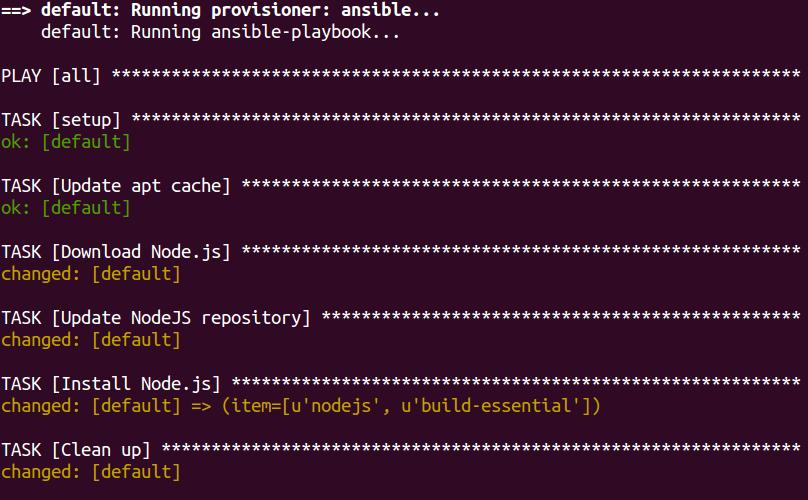
\includegraphics[width=\textwidth]{ansible-running}
  \caption{Ansible tuloste kun se ajaa tehtäviä}
  \label{fig:ansible-running}
\end{figure}

\begin{figure}[h]
  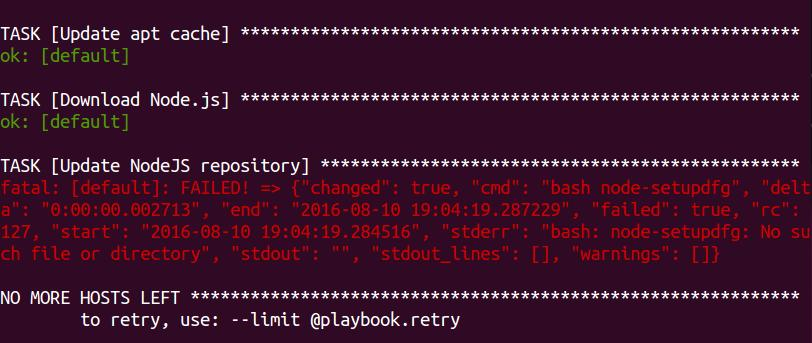
\includegraphics[width=\textwidth]{ansible-fails}
  \caption{Ansiblen tehtävä epäonnistuu}
  \label{fig:ansible-fails}
\end{figure}

\begin{figure}[h]
  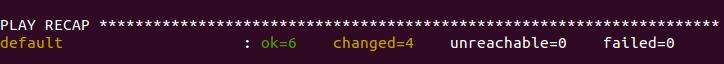
\includegraphics[width=\textwidth]{ansible-summary}
  \caption{Ansiblen yhteenveto tehtävien suorituksesta}
  \label{fig:ansible-summary}
\end{figure}

\begin{lstlisting}[
  label=listing:final-node-vagrantfile,
  language=Ruby,
  caption=Lopullinen Vagrantfile Node virtuaalikoneelle,
  float=h
]
Vagrant.configure(2) do |config|
  config.vm.box = "ubuntu/trusty64"

  config.vm.network "forwarded_port", guest: 8080, host: 3000

  config.vm.synced_folder ".", "/vagrant"

  config.vm.provision "ansible" do |ansible|
    ansible.playbook = "playbook.yml"
  end
end
\end{lstlisting}

\begin{lstlisting}[
  label=listing:node-server,
  language=JavaScript,
  caption=Yksinkertainen Node-palvelin,
  float=h
]
const http = require('http');

const PORT = 8080;

function handleRequest(request, response) {
  response.end(`It Works!! Path Hit: ${request.url}`);
}

const server = http.createServer(handleRequest);

server.listen(PORT, () => {
  console.log(`Server listening on: http://localhost:${PORT}`);
});
\end{lstlisting}

\begin{figure}[h]
  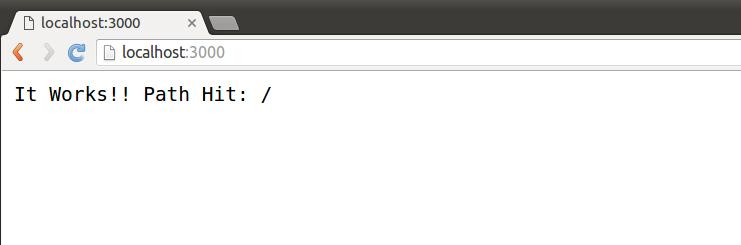
\includegraphics[width=\textwidth]{node-server-response}
  \caption{Node-palvelimen vastaus isäntäkoneessa}
  \label{fig:node-server-response}
\end{figure}

\subsection{Ansible oikeassa maailmassa}

Määrittämällä kaikki playbookin tehtävät yhdessä tiedostossa on yleisesti huono tapa. Tosin asian oppimisen ja yksinkertaisen projektien näkökulmasta siinä ei ole mitään vikaa. Mutta oikeasti playbookin eri tehtävät pitää jaotella erilaisiin rooleihin.

Roolien tarkoitus on jäsentää samaan aiheeseen kuuluvat tehtävät samaan paikkaan. Roolittamisella saadaan helposti uudelleen käytettäviä osioita, joita voidaan käyttää muissakin projekteissa \cite{link:ansible-roles-and-includes}. Esimerkiksi Node halutaan asentaa moneen eri ympäristöön tai projektiin, joten se olisi hyvä jakaa yhteen rooliin.

Roolien uudelleen käytettävyytta voidaan parantaa parametrisoimalla playbookkeja. Esimerkiksi tietokanta ohjelmistoa asentaessa tietokannan portti usein parametrisoidaan. Näin kyseinen rooli voidaan kopioida sellaisenaan toiseen projektiin ja ainoastaan muutetaan tietokannan portti oikeaksi.

\subsection{Ansible roolien käyttäminen}

Seuraavaksi muutetaan aikaisemman virtuaalikoneen playbook roolipohjaiseksi. Lisäksi playbookkiin lisätään MongoDB, joka on suosittu tietokantaohjelma Node-projekteissa. Noden ja MongoDB:n asennus jaetaan erillisiin rooleihin, jotka helpottavat kyseisten ohjelmien uudelleenkäyttöä muissa projekteissa. Lisäksi virtuaalikoneelle annetaan ip-osoite, koska tällöin voidaan ajaa monta virtuaalikonetta yhtä aikaa. Siten voidaan tehdä täydellinen kopio tulevasta tuotantoympäristöstä. Yleisesti tällaisessa ympäristössä esimerkiksi tietokanta on omalla palvelimellaan. Näin voidaan varmistua, että koko järjestelmä toimii, jos paikallisesti ympäristö on mahdollisimman samanlainen.

Ensinksi luodaan projektin juureen ansible-niminen kansio, johon tulee kaikki Ansibleen liittyvät tiedostot. Siirretään playbook.yml tiedosto ansible-kansioon.

Luodaan hosts-tiedosto ansible-kansioon. Hosts-tiedostossa kerrotaan Ansiblelle kaikkien kohdekoneiden tietoja, kuten ip-osoite. Kohdekoneita voidaan myös ryhmitellä hosts-tiedostossa. Esimerkiksi jos tietokantapalvelimia on monta niin ne voidaan nimetä hosts-tiedostossa esimerkiksi databases-ryhmän alle.

Kuviosta \ref{listing:ansible-hosts} nähdään hosts-tiedoston sisältö. Hakasulkeiden sisällä oleva teksti tarkoittaa ryhmää ja sen alapuolella olevat osoitteet ovat kyseisen ryhmän kohdekoneita. Virtuaalikoneelle on nyt keksitty ip-osoite, koska näin voidaan ajaa monta virtuaalikonetta samanaikaisesti. Local-ryhmän alle on annettu keksitty ip-osoite, joka myöhemmin täytyy lisätä myös Vagrantfileen.

\begin{lstlisting}[
  label=listing:ansible-hosts,
  language=bash,
  caption=Hosts-tiedoston sisältö,
  float=h
]
[local]
126.138.117.250
\end{lstlisting}

Seuraavaksi ansible kansioon lisätään ansible.cfg-tiedosto. Tällä tiedostolla voidaan muuttaa joitakin Ansiblen asetuksia, vaikkakin peruskäyttäjille oletusasetukset ovat yleensä riittävät. Tiedoston sisältö näkyy kuviosta \ref{listing:ansible-config}. Tiedostossa kerrotaan mistä Ansiblen täytyy etsiä hosts-tiedostoa. Oletuksena hosts-tiedostoa etsitään polusta \code{etc/ansible/hosts} \cite{link:ansible-inventory}. Kohdekoneet halutaan määrittää projektikohtaisesti ja oletuspolussa oleva hosts-tiedosto ei edes tulisi projektin repositorioon mukaan. Kun käyttää Ansiblen komentoja suoraan komentoriviltä ja haluaa, että Ansibe käyttää tätä cfg-tiedostoa on tärkeää olla samassa kansiossa, jossa cfg-tiedosto on. Muuten Ansible käyttää oletus hosts-tiedostoa.

Nyt Vagrantfileen pitää lisätä asetukset, jotka kertovat Vagrantille  mistä se löytää kohdekoneet, jotka vaativat asennusta. Vagrantfileen lisätään \code{inventory\_path} arvo, joka kertoo missä hosts-tiedosto sijaitsee \cite{link:vagrant-ansible-settings}. Lisäksi annetaan \code{limit} ominaisuuden arvoksi local, joka rajoittaa asennukset kohde koneisiin, jotka kuuluvat ryhmään "local". Myös Vagranfilessä pitää muuttaa playbookin sijainnin polku, koska playbook sijaitsee nyt ansible kansiossa. Lopuksi annetaan virtuaalikoneelle aikaisemmin arvottu ip-osoite. Lopullinen Vagranfile näkyy kuviossa \ref{listing:final-node-vagrantfile-with-roles}.

Viimeiseksi muutetaan playbook.yml tiedostosta hosts-kohdan arvoksi local, koska nyt saatavilla on hosts tiedosto ja haluamme kohdistaa asennuksen vain kohdekoneille, jotka ovat ryhmässä local.

Tässä vaiheessa virtuaalikoneiden asennus on valmisteltu monien virtuaalikoneiden käyttöä varten ja enemmän parhaiden käytäntöjen suuntaan. Seuraavaksi jaotellaan eli ohjelmien asennus rooleihin.

Kaikki roolit pitää olla roles-kansiossa. Sen alle lisätään kansio, jonka nimi on halutunut roolin nimi esimerkiksi: nodejs. Kaikki rooliin liittyvät tehtävät tulevat tasks kansion alle roolin omassa kansiossa. Kaikkien tasks kansioiden tulee sisältää main.yml, joka kokoaa kaikki kyseiseen rooliin liittyvät tehtävät. Siirtymällä ansible kansioon ja ajamalla \code{mkdir -p roles/nodejs/tasks} voidaan luoda kaikki halutut kansiot Nodelle yhdellä kommennolla.

Lisätään tasks kansion alle main.yml tiedosto. Tiedoston sisällöksi leikataan playbook.yml tiedostosta kaikki Noden asentamiseen liittyvät tehtävät. Tehtävien rakennetta ei tarvitse muuttaa, sillä main.yml-tiedostossa voi alkaa suoraa luettelemaan tehtäviä aikaisemmalla rakenteella: nimi ja moduuli.

Seuraavaksi tehdään samat asiat mongodb-roolille. Luodaan sama kansiorakenne ja lisätään main.yml tiedosto. Kuviossa \ref{listing:install-mongo} on kuvattu main.yml-tiedoston sisältö, joka asentaa MongoDB:n.

\begin{lstlisting}[
  label=listing:install-mongo,
  language=Ruby,
  caption=MongoDB:n asennukseen tarvittavat tehtävät,
  float=h
]
---
- name: Import public key used by the package management system
  apt_key:
    keyserver: hkp://keyserver.ubuntu.com:80
    id: 7F0CEB10

- name: Create a list file for MongoDB
  copy:
    content: "deb http://repo.mongodb.org/apt/ubuntu precise/
    mongodb-org/3.0 multiverse"
    dest: /etc/apt/sources.list.d/mongodb-org-3.0.list

- name: Reload local package database
  apt:
    update_cache: yes

- name: Install the MongoDB packages
  apt:
    name: mongodb-org

- name: Make sure MongoDB is started
  service:
    name: mongod
    state: restarted

- name: Add language environment variables
  lineinfile:
    dest: /etc/environment
    line: "{{item}}"
    state: present
  with_items:
    - LANGUAGE="en_US.UTF-8"
    - LANG="en_US.UTF-8"
    - LC_ALL="en_US.UTF-8"

- name: Recompile locale definition files
  locale_gen:
    name: en_US.UTF-8

- name: Reconfigure locales
  command: dpkg-reconfigure locales
\end{lstlisting}

Kaikki roolit ovat nyt luotu joten ne voidaan yhdistää playbookkiin. Playbookkiin lisätään avain "roles" ja sille annetaan lista halutuista rooleista. Lisätään rolesin arvoksi siis nodejs ja mongodb. Kuviossa \ref{listing:playbook-with-roles} näkyy kuinka yksinkertainen playbook on nyt.

Lopullinen projektin ansible kansion rakenne näkyy kuvassa \ref{fig:ansible-folder-structure}. Nyt asennettavien ohjelmien osiot ovat selkeästi erillään toisistaan, jolloin monta kehittäjää voi yhtä aikaa rakentaa ympäristön eri osioita häiritsemättä toisiaan. Lisäksi jos esimerkiksi mongodb rooli halutaan toiseen projektiin voidaan se helposti kopioida.

Nyt ympäristö saadaan jälleen pystyyn kutsumalla \code{vagrant up}. Kun ollaan virtuaalikoneen sisällä kutsutaan \code{mongo}, jolla tarkastetaan, että päästäänkö mongodb-komentoriville. Jos päästään niin mongodb on asennettu oikein. Lisäksi kannattaa kokeilla toimiiko aikaisemmin rakennettu Node-ohjelma vielä. Jos virheitä ei ole tullut missään kohtaa niin ympäristö on onnistuneesti asennettu.

\begin{lstlisting}[
  label=listing:playbook-with-roles,
  language=Ruby,
  caption=Playbook jossa käytetään rooleja,
  float=h
]
---
- hosts: local
  become: true
  remote_user: vagrant
  roles:
    - nodejs
    - mongodb
\end{lstlisting}

\begin{figure}[h]
  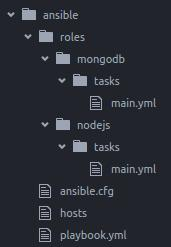
\includegraphics[]{ansible-folder-structure}
  \caption{Ansible kansion rakenne}
  \label{fig:ansible-folder-structure}
\end{figure}

\begin{lstlisting}[
  label=listing:final-node-vagrantfile-with-roles,
  language=Ruby,
  caption=Lopullinen Vagrantfile jossa host-tiedoston sijainti on määritelty,
  float=h
]
Vagrant.configure(2) do |config|
  config.vm.box = "ubuntu/trusty64"

  config.vm.network "private_network", ip: "126.138.117.250"

  config.vm.network "forwarded_port", guest: 8080, host: 3000

  config.vm.synced_folder ".", "/vagrant"

  config.vm.provision "ansible" do |ansible|
    ansible.playbook = "ansible/playbook.yml"
    ansible.limit = "local"
    ansible.inventory_path = "ansible/hosts"
  end
end
\end{lstlisting}

\begin{lstlisting}[
  label=listing:ansible-config,
  language=bash,
  caption=ansible.cfg-tiedoston sisältö,
  float=h
]
[defaults]
inventory = ./hosts
\end{lstlisting}

\subsection{Ansiblen ongelmat}

Vaikka kaikki samoista määrittelyistä tehdyt virtuaalikoneet ovat identtisiä ja niiden pitäisi toimia isäntäkoneesta huolimatta ei ongelmilta kuitenkaan voida välttyä. Windowsilla Ansiblen asennus ei mene täysin suoraviivaisesti. AnsibleWorks:n CTO on kertonut, että Windowssia ei ainakaan lähiaikoina aiota tukea isäntäkoneena Ansiblen kanssa \cite{link:windows-support-for-ansible}.

Windows:lle saa kuitenkin asennettua Ansiblen säätämällä. Yleisin ratkaisu on käyttää Cygwin:ä, jolla saa asennettua unix-pohjaisten järjestelmien paketteja Windowsille \cite{link:cygwin}. Toinen kiertoreitti on asentaa Ansible virtuaalikoneelle. Käytännössä tämä tarkoittaa, että Vagrant provisioi ainoastaan Ansible asennuksen "vagrant up" vaiheessa. Virtuaalikoneen sisälle viedään kaikki Ansible-skriptit. Kun on siirrytty virtuaalikoneen sisälle niin sitten ajetaan Ansible-skriptit. Näin isäntäkoneella ei tarvitse olla asenettuna Ansiblea. Toinen hyvä syy käyttää tätä ratkaisua on sitoa Ansiblen asennus tiettyy versioon, jolloin Ansiblenkin versio on aina sama. Tällöin esimerkiksi jos Ansible muuttaa moduuleita vanhat skriptit eivät voi mennä rikki.

Muista kertoa ansiblen sivusta galaxy.ansible.com